\documentclass[11pt]{article}
\usepackage{fontspec}
\setmainfont{DejaVu Serif}
\setsansfont{DejaVu Sans}
\usepackage{polyglossia}
\setmainlanguage{greek}
\setotherlanguage{english}
\tolerance=2500
\emergencystretch=3em   % safety net so justified lines never overflow the margin
\usepackage{amsmath,amssymb}
\usepackage{geometry}\geometry{margin=2.4cm}
\usepackage{xcolor}\usepackage{graphicx}
\usepackage{booktabs}
\usepackage{caption}\captionsetup{font=small,labelfont=bf}
\usepackage[hidelinks]{hyperref}
\graphicspath{{figures/}}

\definecolor{ink}{HTML}{16212e}\definecolor{accent}{HTML}{1f5fa8}\definecolor{soft}{HTML}{eef3fb}
\definecolor{warn}{HTML}{a8341f}\definecolor{good}{HTML}{1f7a44}
\color{ink}
\newcommand{\eur}{€}
\newcommand{\aside}[1]{\par\medskip\noindent\colorbox{soft}{\parbox{\dimexpr\linewidth-2\fboxsep}{#1}}\par\medskip}
\setlength{\parskip}{0.45em}\setlength{\parindent}{0pt}
\usepackage{titlesec}
\titleformat{\section}{\large\bfseries\color{accent}}{\thesection.}{0.5em}{}
\titleformat{\subsection}{\normalsize\bfseries}{}{0em}{}

\newcommand{\paperref}{\emph{«From Dead Cross-Sectional Momentum to Belief-State Deep Time-Series
Momentum: An Honest, Cost-Aware Study on a Diversified Asset Basket»} (Drakos 2026)}

\begin{document}

% ===================== ΕΞΩΦΥΛΛΟ =====================
\begin{titlepage}\centering
\thispagestyle{empty}
\vspace*{3.2cm}
{\sffamily\bfseries\fontsize{52}{56}\selectfont QUANTIQ}\\[14pt]
{\sffamily\fontsize{22}{26}\selectfont\color{accent} Deep Learning Trading}\\[3.4cm]
\rule{0.66\linewidth}{0.4pt}\\[18pt]
{\large\bfseries Διαφοροποιημένη στρατηγική συναλλαγών παρακολούθησης τάσεων}\\[8pt]
{\normalsize Τεχνική και επιχειρηματική επισκόπηση: μεθοδολογία, ζωντανή λειτουργία στο eToro\\
και αποτελέσματα ελέγχων σε πραγματικά δεδομένα}\\[14pt]
\rule{0.66\linewidth}{0.4pt}
\vfill
{\large\bfseries Dr.\ Stefanos Drakos}\\[5pt]
{\normalsize QUANTIQ \,/\, AGEL AI}\\[3pt]
{\small Ιούνιος 2026}
\end{titlepage}

% ===================== ΕΙΣΑΓΩΓΗ =====================
\noindent
Το παρόν κείμενο απευθύνεται σε επιχειρηματικά στελέχη και επενδυτές που επιθυμούν να κατανοήσουν, χωρίς
τεχνική ορολογία αλλά και χωρίς υπεραπλουστεύσεις, το σύστημα συναλλαγών που αναπτύξαμε για την πλατφόρμα
QUANTIQ. Πρόκειται για μια αυτοματοποιημένη στρατηγική η οποία λαμβάνει επενδυτικές αποφάσεις με βάση
ποσοτικά κριτήρια και μεθόδους βαθιάς μάθησης, και η οποία προορίζεται να λειτουργεί απευθείας πάνω στον
λογαριασμό eToro του χρήστη.

Στόχος της παρουσίασης είναι η τεκμηριωμένη και ειλικρινής εικόνα: τι ακριβώς κάνει το σύστημα, σε ποια
επιστημονικά θεμέλια στηρίζεται, ποια αποτελέσματα έχει αποδώσει σε ελέγχους με πραγματικά δεδομένα της
αγοράς, και ποια είναι τα όρια και οι κίνδυνοί του. Η πλήρης μεθοδολογία τεκμηριώνεται στην ερευνητική
εργασία \paperref. Όλα τα μεγέθη που παρατίθενται είναι \textbf{καθαρά μετά το κόστος συναλλαγών} και
προέρχονται από χρονικές περιόδους \textbf{εκτός του δείγματος εκπαίδευσης} του μοντέλου, ώστε να
αποτυπώνουν ρεαλιστικά την αναμενόμενη συμπεριφορά και όχι μια εκ των υστέρων προσαρμογή στα δεδομένα.

\section{Τι κάνει το σύστημα}

Το σύστημα εφαρμόζει μια πειθαρχημένη στρατηγική παρακολούθησης τάσεων (trend following). Για κάθε
χρηματοοικονομικό προϊόν εξετάζει, με ποσοτικά κριτήρια, αν η τιμή κινείται ανοδικά ή καθοδικά κατά τους
προηγούμενους μήνες. Όταν η τάση είναι ανοδική, ανοίγει θέση αγοράς· όταν είναι καθοδική, παραμένει εκτός
ή, εφόσον αυτό επιτραπεί, λαμβάνει θέση πώλησης (short). Το μέγεθος κάθε θέσης ορίζεται αντιστρόφως
ανάλογο της μεταβλητότητας του προϊόντος, ώστε κανένα μεμονωμένο προϊόν να μην κυριαρχεί στο συνολικό
ρίσκο του χαρτοφυλακίου. Η σύνθεση των θέσεων αναπροσαρμόζεται μία φορά τον μήνα.

Εξίσου κρίσιμο είναι ότι το σύστημα δεν επενδύει σε ένα μόνο προϊόν, αλλά σε ένα \textbf{διαφοροποιημένο
καλάθι περιουσιακών στοιχείων με χαμηλή μεταξύ τους συσχέτιση}: μετοχικούς δείκτες, ομόλογα, χρυσό,
πετρέλαιο, το δολάριο και, προαιρετικά, κρυπτονομίσματα. Επειδή τα στοιχεία αυτά δεν κινούνται
ταυτόχρονα, οι απώλειες του ενός αντισταθμίζονται συχνά από τα υπόλοιπα, περιορίζοντας τις απότομες
πτώσεις του κεφαλαίου. Η διαφοροποίηση χαμηλά συσχετισμένων στοιχείων είναι το μοναδικό δομικό
πλεονέκτημα που προσφέρεται ουσιαστικά χωρίς κόστος στις αγορές, και αποτελεί τον ακρογωνιαίο λίθο της
προσέγγισής μας.

\section{Πώς το μοντέλο μαθαίνει}

Έχουμε δύο εκδοχές, και οι δύο μαθαίνουν από δεκαεπτά χρόνια πραγματικού ιστορικού (δωρεάν δεδομένα
Yahoo, που έχουν αρκετό βάθος για σωστή εκπαίδευση). Η πρώτη, που τη λέμε \emph{rules}, ακολουθεί έναν
σταθερό μαθηματικό κανόνα τάσης: είναι απλή, διάφανη, χωρίς «μαύρο κουτί». Η δεύτερη είναι ένα
\emph{νευρωνικό δίκτυο} (LSTM) που μαθαίνει μόνο του το σχήμα της τάσης από δέκα πληροφορίες ανά προϊόν.

Αξίζει να πω ποιες είναι αυτές οι δέκα πληροφορίες, γιατί εκεί κρύβεται η ουσία. Δεν δίνουμε στο μοντέλο
τη γυμνή τιμή. Του δίνουμε πέντε διαφορετικές «αποδόσεις» --- από περίπου έναν μήνα μέχρι έναν χρόνο ---
καθεμία διαιρεμένη με τη νευρικότητα του προϊόντος, ώστε να ξεχωρίζει η πραγματική τάση από τον θόρυβο.
Του δίνουμε τη μεταβλητότητα, δηλαδή πόσο αναστατωμένο είναι το προϊόν αυτή τη στιγμή. Του δίνουμε τρεις
δείκτες από ένα φίλτρο Kalman που εκτιμά την «ταχύτητα» της τάσης και πόσο αξιόπιστη είναι. Και τέλος,
του δίνουμε ένα σήμα από έναν ανιχνευτή που λέγεται BOCPD, ο οποίος χτυπάει καμπανάκι όχι όταν απλώς
πέφτει μια τιμή, αλλά όταν αλλάζει η ίδια η \emph{συμπεριφορά} της αγοράς. Τον σκέφτομαι σαν ένα έξυπνο
φρένο που πατιέται στις πραγματικές αλλαγές καθεστώτος, όχι στον κάθε μικρό τρόμο.

Το πιο σημαντικό στην εκπαίδευση είναι ότι αποφεύγουμε την «κλεψιά». Χρησιμοποιούμε μια αυστηρή μέθοδο
(nested walk-forward) όπου το μοντέλο μαθαίνει αποκλειστικά από το παρελθόν και δοκιμάζεται σε μέλλον
που δεν έχει δει, βήμα-βήμα. Γι' αυτό τα νούμερα που ακολουθούν είναι έντιμα και όχι «ζωγραφισμένα»
πάνω στα δεδομένα.

\begin{figure}[ht]\centering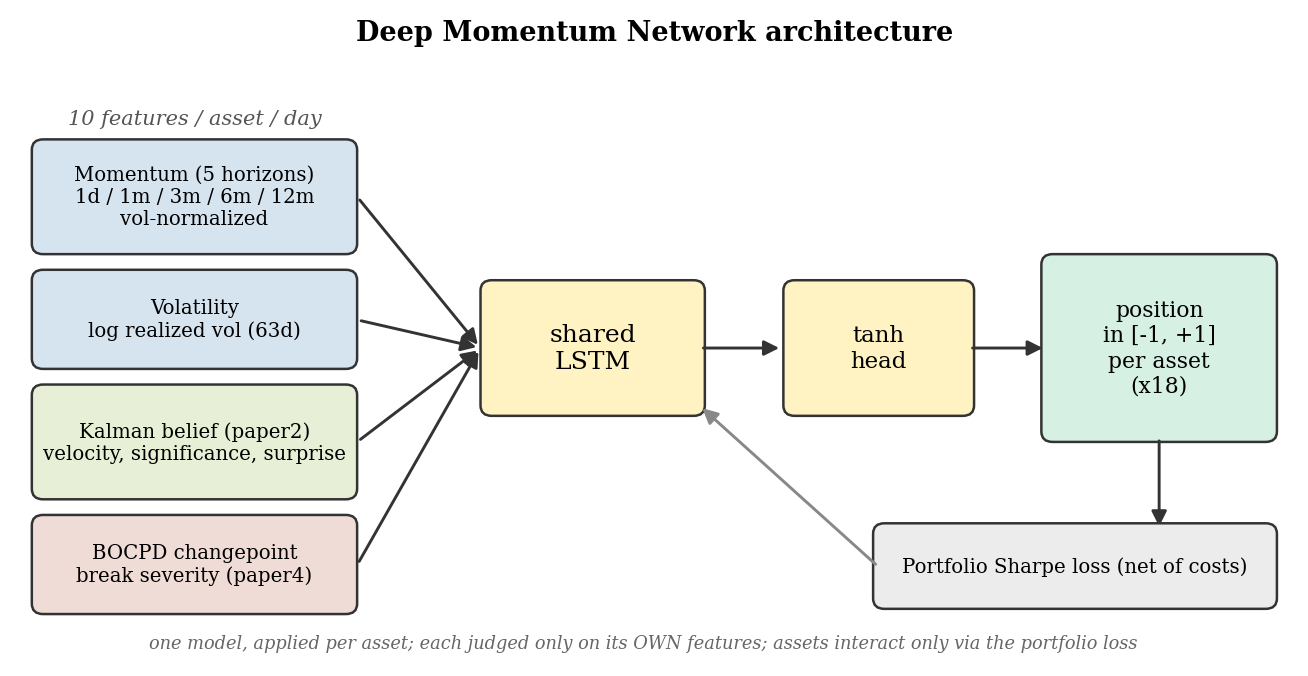
\includegraphics[width=.74\linewidth]{fig_architecture.png}
\caption{Πώς αποφασίζει το νευρωνικό μοντέλο: δέκα πληροφορίες για κάθε προϊόν μπαίνουν στο δίκτυο, και
βγαίνει μια θέση από $-1$ (πλήρης πώληση) έως $+1$ (πλήρης αγορά).}\end{figure}

\section{Από την εκπαίδευση στο eToro}

Η λογική είναι «μάθε βαθιά, δούλεψε ζωντανά»: το μοντέλο εκπαιδεύεται στα βαθιά δεδομένα Yahoo, αλλά
όταν τρέχει στο QUANTIQ διαβάζει τις \textbf{πραγματικές τιμές και τα προϊόντα του eToro}. Κάθε φορά που
το καλούμε, ακολουθεί τέσσερα βήματα. Πρώτα υπολογίζει την επιθυμητή θέση για κάθε προϊόν. Μετά βρίσκει
το καθένα μέσα στο eToro με αυτόματη αναζήτηση· ό,τι δεν υπάρχει εκεί το παραλείπει και μοιράζει ξανά το
κεφάλαιο στα διαθέσιμα, ώστε να μένει πλήρως επενδυμένο σε αυτά που πραγματικά μπορούμε να αγοράσουμε.
Έπειτα συγκρίνει με ό,τι έχουμε ήδη ανοιχτό και φτιάχνει τη λίστα των εντολών, αγνοώντας ασήμαντες
αλλαγές. Και τέλος, μόνο αν δώσουμε ρητή εντολή, στέλνει τις εντολές στον \textbf{demo} λογαριασμό.
Χωρίς αυτή την εντολή, το σύστημα απλώς μας δείχνει τι θα έκανε.

Μια εύλογη απορία είναι πότε κλείνει μια θέση. Δεν βάζουμε stop-loss. Μια θέση κλείνει ή μικραίνει στο
μηνιαίο ξανα-ζύγισμα, όταν η τάση του προϊόντος γυρίσει ή αδυνατίσει --- ή νωρίτερα, αν ο ανιχνευτής
αλλαγής δει ότι κάτι άλλαξε ουσιαστικά. Παρακάτω εξηγώ γιατί το stop-loss, που ακούγεται λογικό,
αποδείχθηκε στην πράξη ζημιογόνο.

Τέλος, υπάρχει ένα «κουμπί ρίσκου». Διαλέγουμε πόση ετήσια μεταβλητότητα θέλουμε --- ας πούμε 10\% για
συντηρητικά ή 20\% για πιο τολμηρά --- και το σύστημα μοχλεύει ανάλογα ώστε να την πετύχει. Για να ξέρει
πόσο νευρικό είναι το καλάθι τη δεδομένη στιγμή, μετράει τη μεταβλητότητα με ένα κυλιόμενο παράθυρο των
τελευταίων περίπου εξήντα τριών ημερών, χωρίς ποτέ να κοιτάει το μέλλον, κι έτσι είναι κατάλληλο για
ζωντανή χρήση. Υπάρχει και μια ταχύτερη παραλλαγή (EWMA) που δίνει μεγαλύτερη βαρύτητα στις πρόσφατες
μέρες· τη συγκρίνω με την κλασική λίγο πιο κάτω.

\aside{\textbf{Ασφάλεια.} Η προεπιλογή είναι να μη στέλνεται τίποτα· βλέπουμε απλώς το σχέδιο. Η
εκτέλεση γίνεται μόνο στον demo λογαριασμό σε αυτή τη φάση. Δεν πρόκειται για αυτόματο trader ---
τον έλεγχο τον έχει ο άνθρωπος.}

\section{Το βασικό τεστ: πραγματικές τιμές eToro}

Το πιο τίμιο τεστ που μπορούσαμε να κάνουμε ήταν να τρέξουμε τη στρατηγική πάνω στις \textbf{πραγματικές
ημερήσιες τιμές του eToro}, στα ίδια προϊόντα που θα αγόραζε κανείς. Πήραμε πέντε όσο γίνεται πιο
διαφορετικά πράγματα --- τον δείκτη μετοχών SPY, τα ομόλογα TLT, τον χρυσό GLD, το πετρέλαιο USO και το
δολάριο UUP --- και αφήσαμε το μοντέλο να δουλέψει μόνο με αγορές, στο 10\% ρίσκο, για περίπου τρία
χρόνια. Τα 10.000\eur{} έγιναν 15.073\eur{}, δηλαδή περίπου $+50\%$ μετά τα κόστη, με τη χειρότερη
βουτιά του λογαριασμού να μην ξεπερνά το 9\%. Η «ποιότητα» του κέρδους, που τη μετράμε με τον δείκτη IR,
βγήκε 1.42 --- και οτιδήποτε πάνω από το 1.0 θεωρείται πολύ καλό.

\begin{table}[ht]\centering\small
\begin{tabular}{lrl}\toprule
Μέτρο & Αποτέλεσμα & Τι σημαίνει \\\midrule
10.000\eur{} έγιναν & \textcolor{good}{\textbf{15.073\eur{}}} & $+50\%$ σε $\sim$3 χρόνια, μετά κόστη \\
IR (ποιότητα) & \textcolor{good}{$+1.42$} & πάνω από 1.0 = πολύ καλό \\
Χειρότερη πτώση & \textcolor{warn}{$-9\%$} & το χειρότερο βύθισμα από την κορυφή \\
\bottomrule\end{tabular}
\caption{Πέντε διαφοροποιημένα προϊόντα, μόνο αγορές, 10\% ρίσκο, σε πραγματικές τιμές eToro (2023--2026).}
\end{table}

\begin{figure}[ht]\centering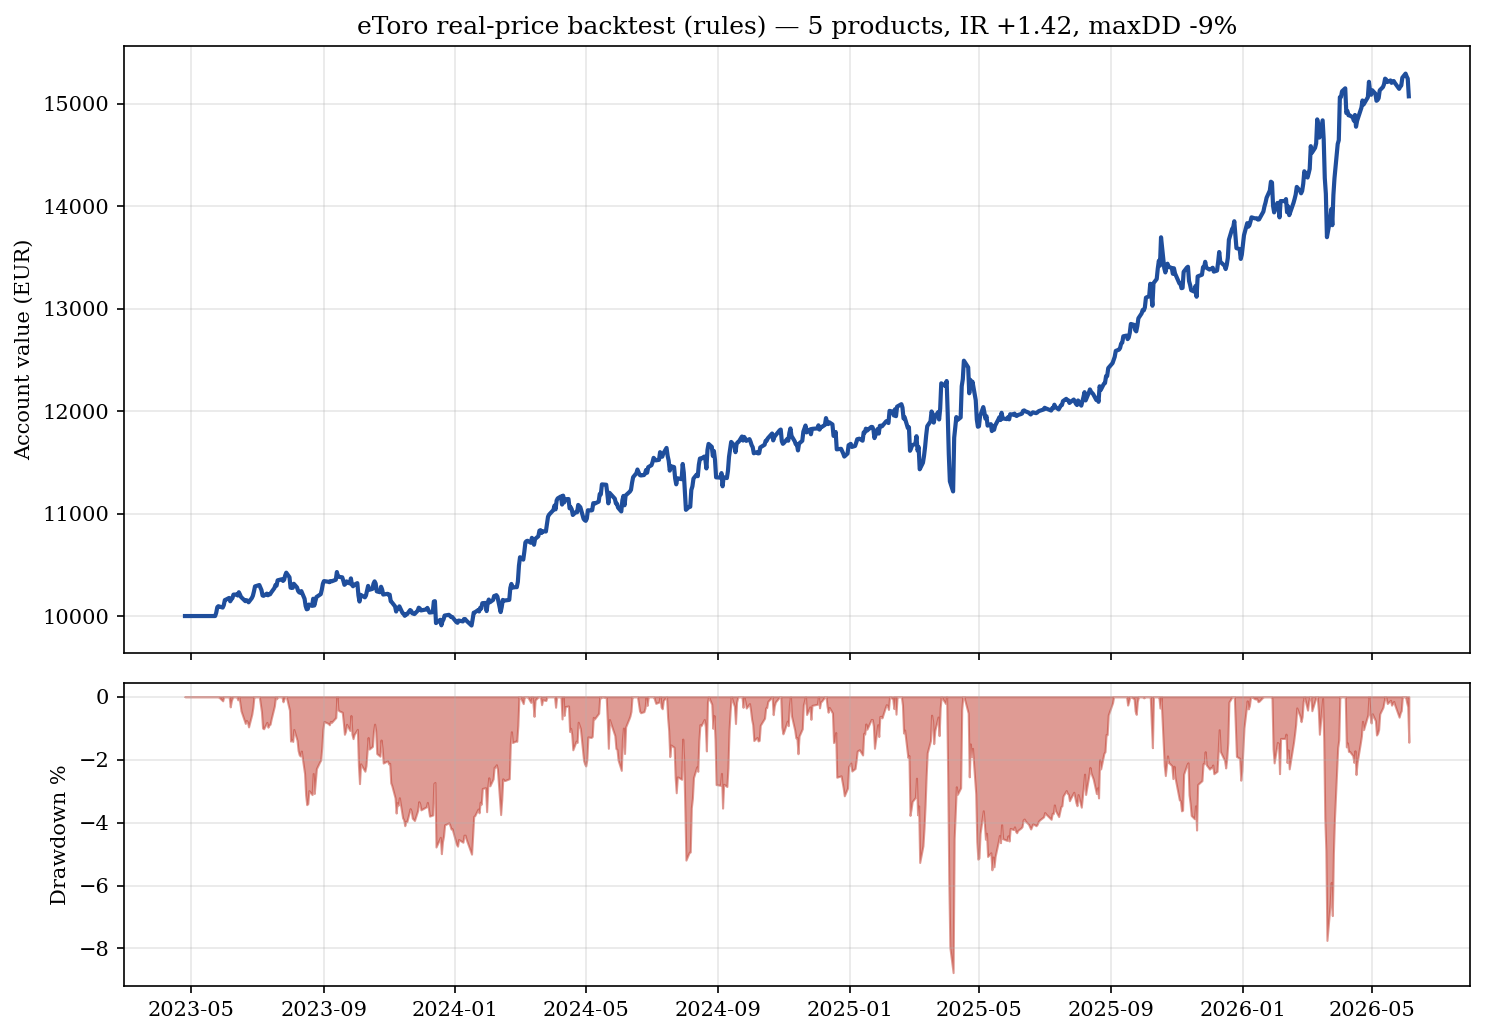
\includegraphics[width=.92\linewidth]{fig_etoro_backtest.png}
\caption{Η εξέλιξη του λογαριασμού. Πάνω, πώς μεγάλωσαν τα 10.000\eur{}· κάτω, με κόκκινο, πόσο κάτω από
την κορυφή του βρισκόταν κάθε στιγμή --- ποτέ περισσότερο από 9\%.}\end{figure}

\section{Λίγα ή πολλά προϊόντα;}

Ένα από τα πιο χρήσιμα πράγματα που μάθαμε είναι ότι τα περισσότερα προϊόντα δεν σημαίνουν καλύτερο
αποτέλεσμα. Δοκιμάσαμε και ένα ευρύ καλάθι δεκαεπτά ETF, και βγήκε \emph{χειρότερο} από τα πέντε. Ο
λόγος είναι απλός: τα δεκαεπτά είχαν πολλά που έμοιαζαν μεταξύ τους (πολλοί δείκτες μετοχών που κινούνται
παρέα), οπότε η πραγματική διαφοροποίηση ήταν λιγότερη απ' όσο φαινόταν. Πέντε αληθινά διαφορετικά
πράγματα έδωσαν καλύτερη ποιότητα κέρδους και, ταυτόχρονα, μικρότερη βουτιά.

\begin{table}[ht]\centering\small
\begin{tabular}{lrrr}\toprule
Καλάθι & IR & Χειρ. πτώση & 10.000\eur{} $\to$ \\\midrule
17 ETF, αγορές και πωλήσεις & $+0.60$ & $-14\%$ & 11.804\eur{} \\
17 ETF, μόνο αγορές & $+1.03$ & $-15\%$ & 13.409\eur{} \\
\textbf{5 διαφοροποιημένα, μόνο αγορές} & \textcolor{good}{\textbf{$+1.42$}} & $-9\%$ & \textcolor{good}{\textbf{15.073\eur{}}} \\
\bottomrule\end{tabular}
\caption{Λιγότερα αλλά πραγματικά διαφορετικά προϊόντα κερδίζουν τα πολλά και όμοια.}
\end{table}

\section{Ο πίνακας συσχέτισης: η απόδειξη της διαφοροποίησης}

Το προηγούμενο εύρημα δεν είναι θέμα γούστου· μετριέται. Το κατάλληλο εργαλείο είναι ο
\textbf{πίνακας συσχέτισης} των ημερήσιων αποδόσεων: δείχνει, για κάθε ζεύγος προϊόντων, πόσο κινούνται
μαζί (τιμή κοντά στο $+1$) ή αντίθετα (κοντά στο $-1$). Δύο προϊόντα με συσχέτιση γύρω στο $0{,}9$
είναι, πρακτικά, \emph{ένα} στοίχημα γραμμένο δύο φορές: προσθέτουν συναλλαγές και κόστος χωρίς να
προσθέτουν ουσιαστική διαφοροποίηση. Συμπυκνώνουμε την εικόνα σε έναν αριθμό, τον \textbf{αριθμό
πραγματικά ανεξάρτητων στοιχημάτων}: ισούται με το πλήθος των προϊόντων αν είναι όλα ασυσχέτιστα, και
καταρρέει προς το ένα όσο αυτά κινούνται μαζί.

Εφαρμοσμένο στις πραγματικές τιμές eToro, το αποτέλεσμα είναι αποκαλυπτικό. Το καλάθι των πέντε
διαφοροποιημένων προϊόντων έχει χαμηλή μέση συσχέτιση και διατηρεί σχεδόν όλη τη διαφοροποίησή του· το
ευρύ καλάθι των δεκαεπτά, αντιθέτως, καταρρέει σε λιγότερα από τέσσερα πραγματικά στοιχήματα --- δηλαδή
\emph{λιγότερα} από όσα προσφέρουν τα πέντε. Αυτή ακριβώς είναι η αιτία πίσω από το «πέντε καλύτερα από
δεκαεπτά».

\begin{table}[ht]\centering\small
\begin{tabular}{lrr}\toprule
Καλάθι & Μέση \textbar συσχέτιση\textbar & Πραγματικά ανεξάρτητα στοιχήματα \\\midrule
\textbf{5 διαφοροποιημένα} & \textcolor{good}{$0{,}19$} & \textcolor{good}{\textbf{4{,}2 / 5}} \,(84\%) \\
17 ETF & \textcolor{warn}{$0{,}38$} & \textcolor{warn}{\textbf{3{,}9 / 17}} \,(23\%) \\
\bottomrule\end{tabular}
\caption{Όσο χαμηλότερη η μέση συσχέτιση, τόσο περισσότερη η πραγματική διαφοροποίηση. Τα δεκαεπτά
προϊόντα μετρούν λιγότερα ανεξάρτητα στοιχήματα από τα πέντε.}
\end{table}

\begin{figure}[ht]\centering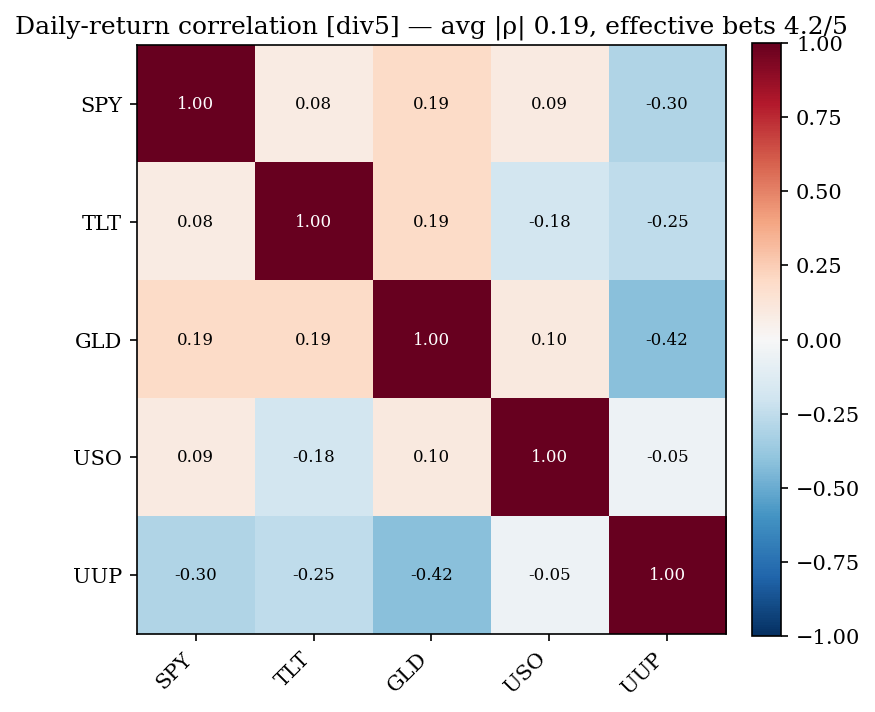
\includegraphics[width=.66\linewidth]{fig_correlation_div5.png}
\caption{Τα πέντε διαφοροποιημένα προϊόντα. Σχεδόν όλα τα κελιά είναι ωχρά (χαμηλή συσχέτιση)· το
δολάριο (UUP) κινείται \emph{αντίθετα} από τα υπόλοιπα ($-0{,}42$ με τον χρυσό), λειτουργώντας ως
ασπίδα.}\end{figure}

\begin{figure}[ht]\centering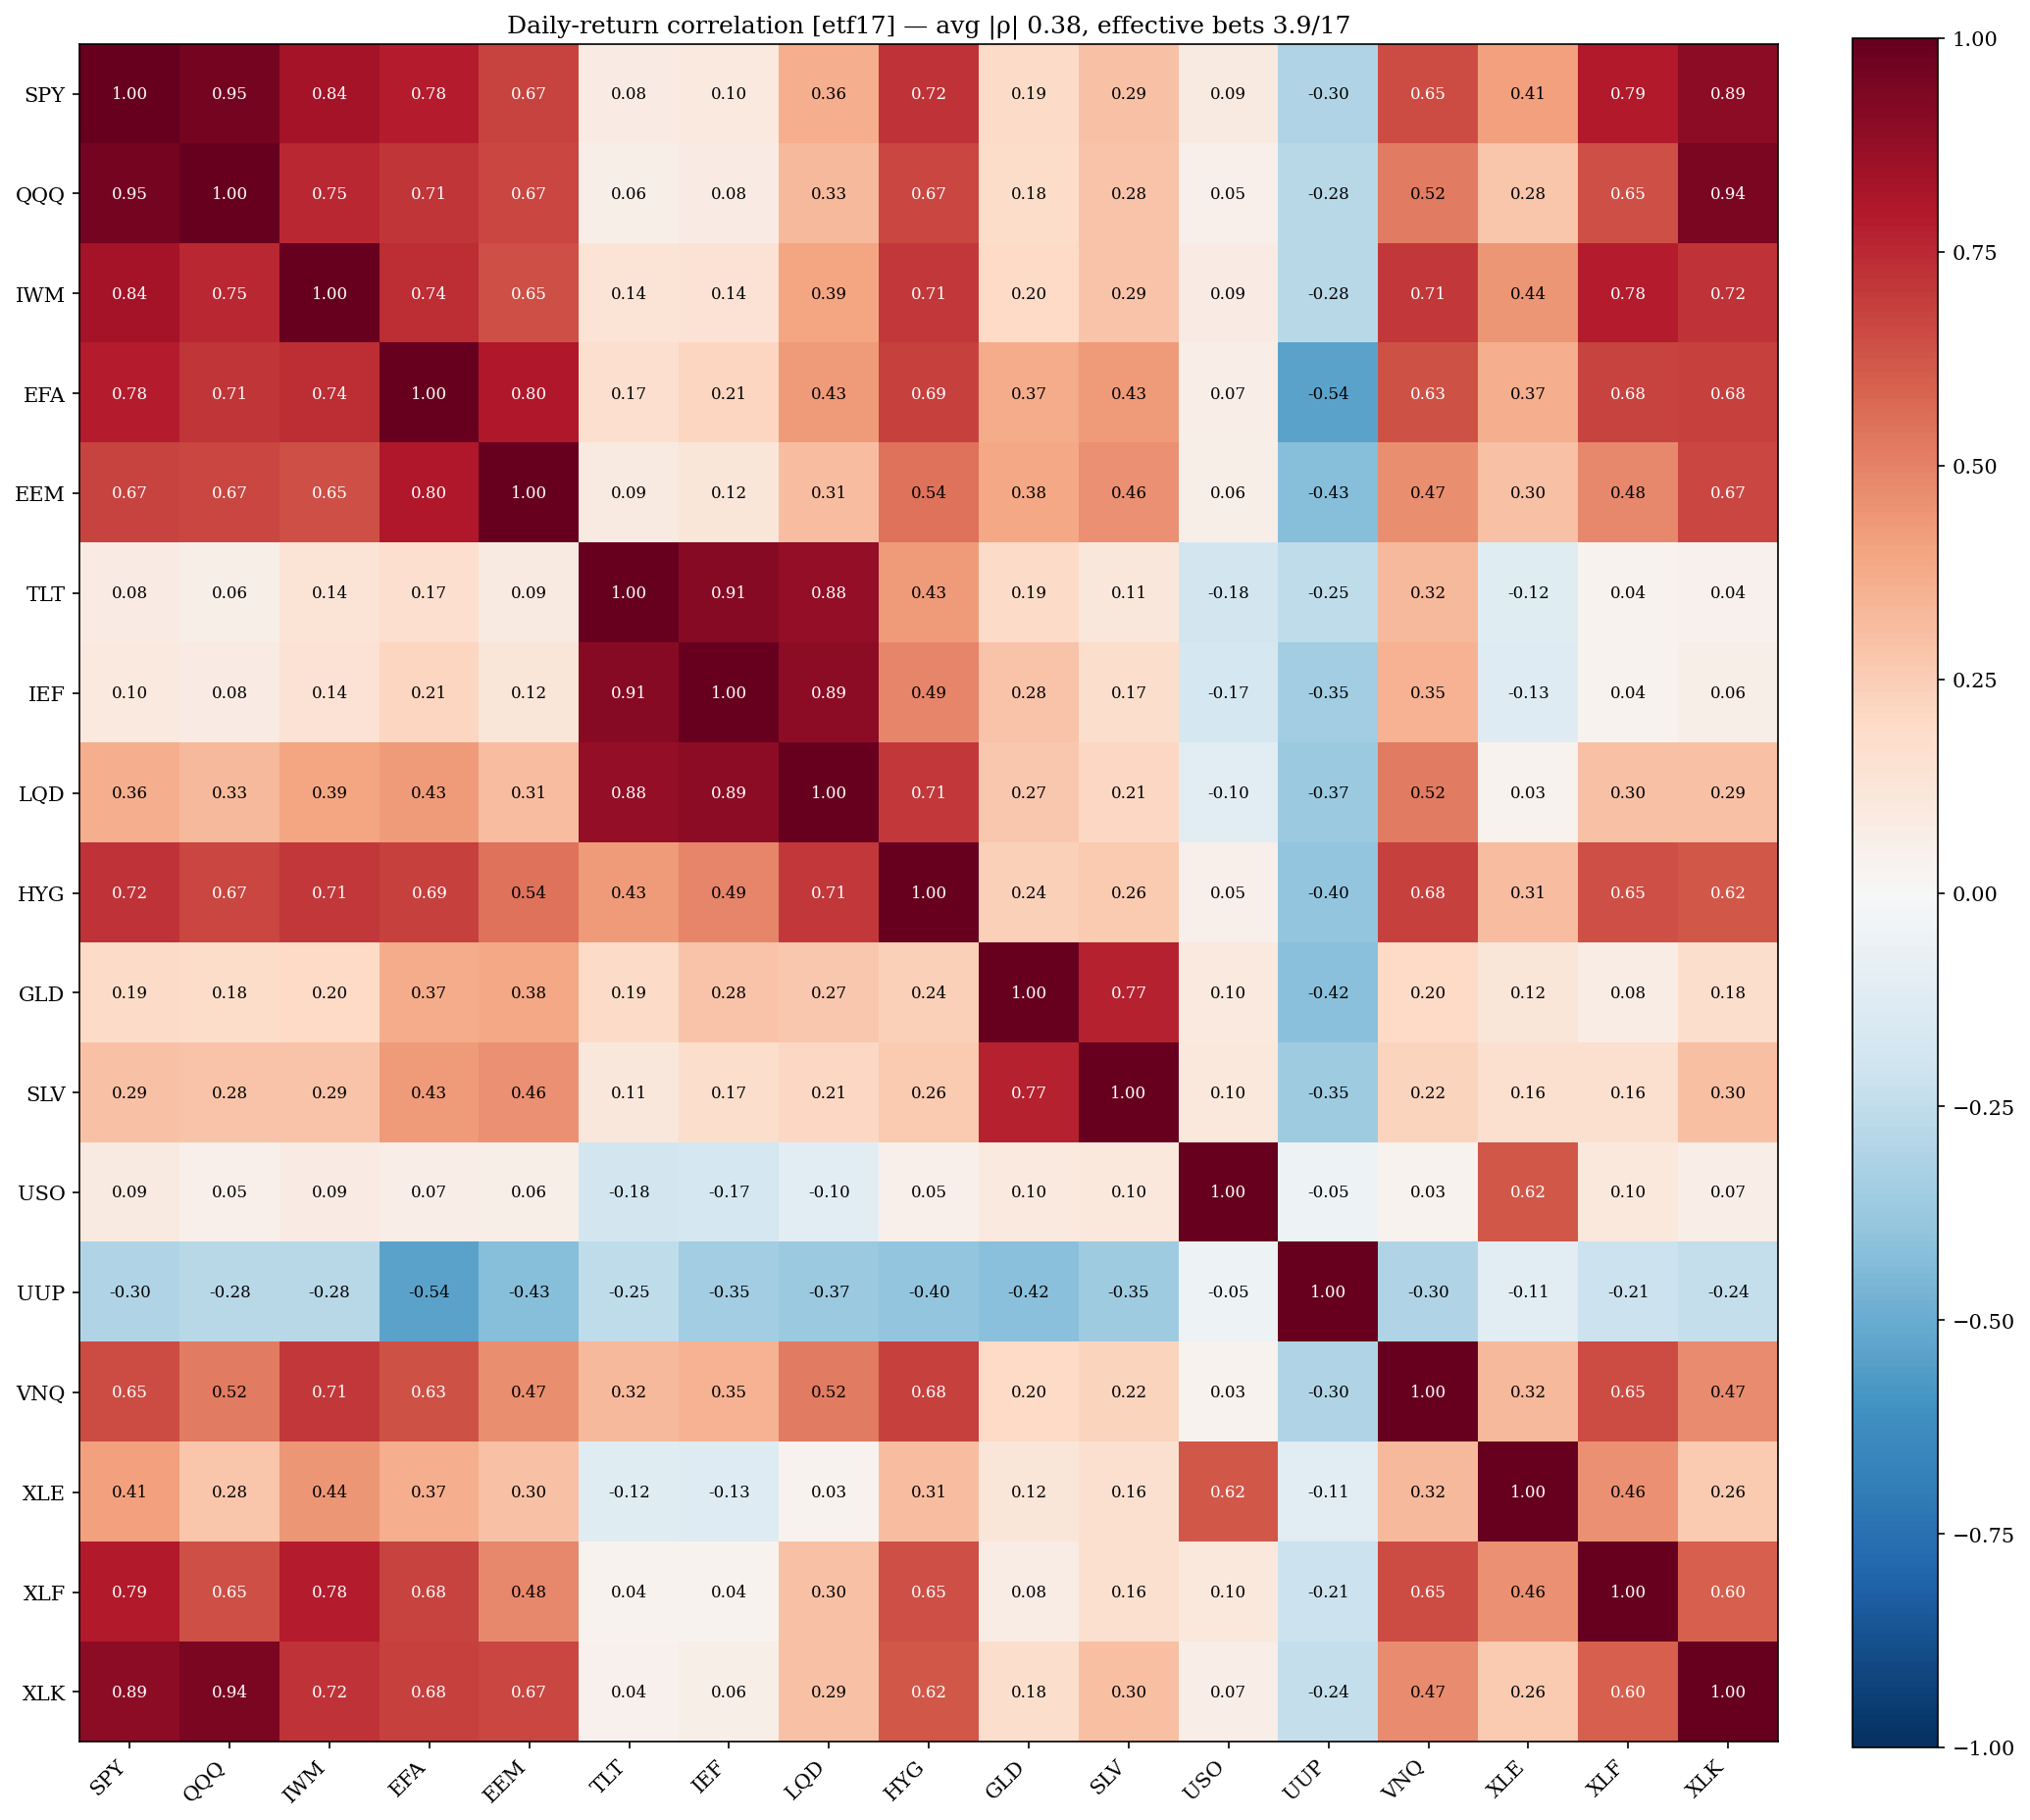
\includegraphics[width=.82\linewidth]{fig_correlation_etf17.png}
\caption{Τα δεκαεπτά ETF. Το έντονο κόκκινο τετράγωνο πάνω αριστερά είναι μια ομάδα μετοχικών δεικτών
που κινούνται σχεδόν ταυτόσημα --- ένα στοίχημα γραμμένο πολλές φορές. Γι' αυτό ο αριθμός πραγματικών
στοιχημάτων μένει χαμηλός παρά το πλήθος.}\end{figure}

\section{Μόνο αγορές ή και πωλήσεις;}

Όταν επιτρέπουμε και πωλήσεις (short), το μοντέλο μπορεί να βγάλει κέρδος και από τις πτώσεις. Σε αυτή
τη συγκεκριμένη, ανοδική περίοδο όμως οι θέσεις πώλησης ήταν περισσότερο βάρος παρά όφελος, κι έτσι η
εκδοχή «μόνο αγορές» βγήκε καλύτερη. Δεν είναι όμως πάντα έτσι: σε ένα κραχ συμβαίνει το αντίθετο, γιατί
οι πωλήσεις τότε προστατεύουν. Με άλλα λόγια, οι πωλήσεις είναι σαν ασφάλεια --- πληρώνεις λίγο κέρδος
σε καλές εποχές για να έχεις προστασία στις κακές.

\begin{figure}[ht]\centering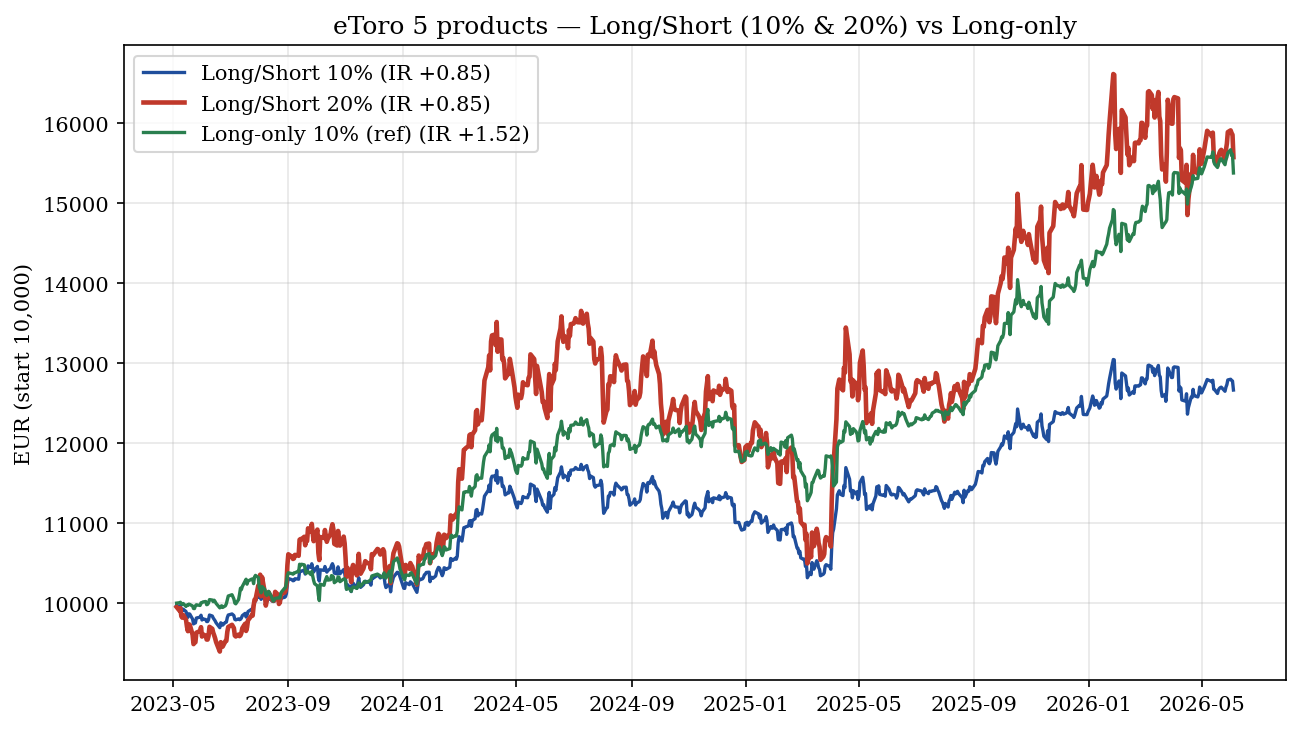
\includegraphics[width=.88\linewidth]{fig_etoro_5_longshort.png}
\caption{Οι δύο προσεγγίσεις στα ίδια πέντε προϊόντα. Το «μόνο αγορές» στο 10\% (πράσινο) φτάνει σχεδόν
ίδιο τέλος με το «αγορές και πωλήσεις» στο 20\%, αλλά με τη μισή βουτιά. Το δεύτερο όμως κρατά την
προστασία σε κραχ που το πρώτο χάνει.}\end{figure}

\section{Με λίγο crypto}

Επειδή το Bitcoin υπάρχει στο eToro, δοκιμάσαμε να βάλουμε κι αυτό στο καλάθι. Είναι γνωστό για την
αγριότητά του, αλλά εδώ ακριβώς φαίνεται η ομορφιά του κανόνα «νευρικό προϊόν, μικρή θέση»: το σύστημα
του δίνει αυτόματα μικρό βάρος, οπότε προσθέτει διαφοροποίηση χωρίς να ανεβάζει το συνολικό ρίσκο. Το
αποτέλεσμα ήταν IR 1.29 με χειρότερη πτώση μόλις 7\%.

\begin{figure}[ht]\centering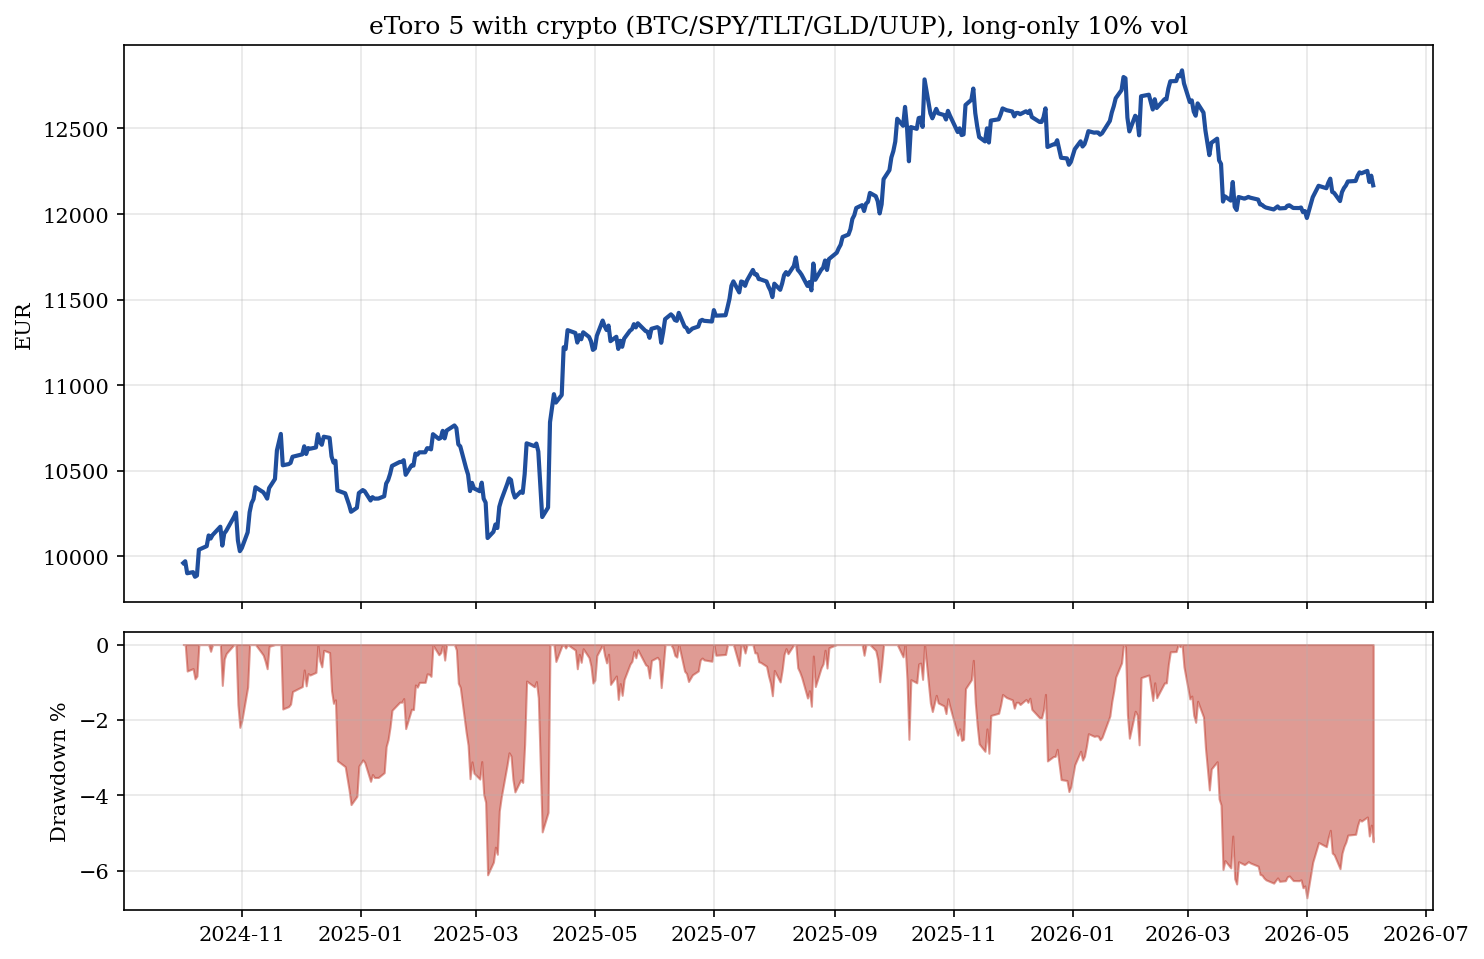
\includegraphics[width=.82\linewidth]{fig_etoro_crypto5.png}
\caption{Καλάθι με Bitcoin και διαφοροποιητές. Η μικρή, αυτόματα ρυθμισμένη θέση στο BTC κρατά χαμηλή
τη βουτιά διατηρώντας καλή ποιότητα κέρδους.}\end{figure}

\section{Το κουμπί ρίσκου}

Θέλω να είμαι ξεκάθαρος σε κάτι που συχνά παρεξηγείται: το κέρδος είναι ανάλογο του ρίσκου που διαλέγει
κανείς, και δεν υπάρχει τρόπος να το παρακάμψεις. Αν ανεβάσεις το κουμπί, ανεβαίνουν \emph{και} το
κέρδος \emph{και} οι βουτιές, σχεδόν στην ίδια αναλογία. Η ποιότητα του κέρδους μένει ίδια· αλλάζει μόνο
το μέγεθος. Ο παρακάτω πίνακας το δείχνει καθαρά πάνω στα πραγματικά δεδομένα.

\begin{table}[ht]\centering\small
\begin{tabular}{lrrr}\toprule
Επίπεδο ρίσκου & Κέρδος (3 χρ.) & Ανά έτος & Χειρ. πτώση \\\midrule
10\% (συντηρητικό) & $+30\%$ & $+9\%$ & $-15\%$ \\
15\% & $+46\%$ & $+13\%$ & $-22\%$ \\
20\% & $+63\%$ & $+18\%$ & $-28\%$ \\
30\% (επιθετικό) & \textcolor{good}{$+98\%$} & $+26\%$ & \textcolor{warn}{$-40\%$} \\
\bottomrule\end{tabular}
\caption{Όσο ανεβαίνει το ρίσκο, ανεβαίνουν μαζί κέρδος και βουτιά. Δεν υπάρχει απόδοση χωρίς ανάλογο ρίσκο.}
\end{table}

\begin{figure}[ht]\centering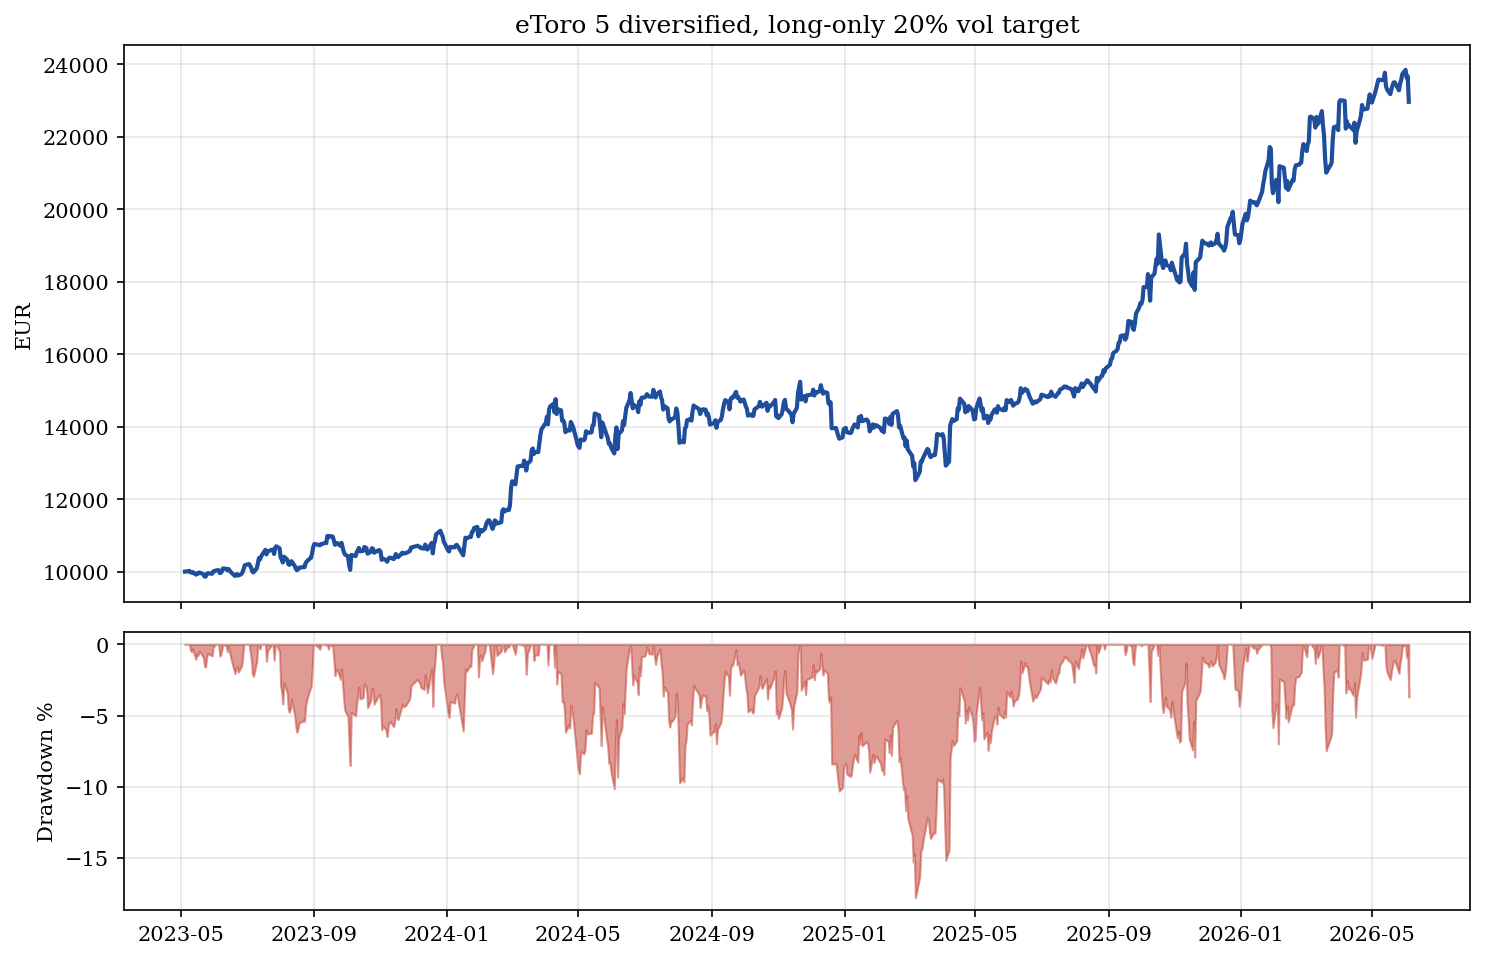
\includegraphics[width=.82\linewidth]{fig_etoro_5_vol20.png}
\caption{Τα ίδια πέντε προϊόντα στο 20\% ρίσκο: διπλάσιο κέρδος (10.000\eur{} $\to$ 22.958\eur{}) αλλά
και διπλάσια βουτιά σε σχέση με το 10\%.}\end{figure}

\section{Πώς μετράμε τη νευρικότητα του καλαθιού}

Το κουμπί ρίσκου χρειάζεται να ξέρει πόσο νευρικό είναι το καλάθι τώρα, και αυτό μπορεί να μετρηθεί με
περισσότερους από έναν τρόπους. Συγκρίναμε τρεις πάνω στα ίδια ακριβώς δεδομένα. Ο πρώτος, ο «στατικός»,
παίρνει έναν μέσο όρο όλης της περιόδου και χρησιμεύει μόνο για εικόνα. Ο δεύτερος, ο κυλιόμενος των
εξήντα τριών ημερών, είναι αυτός που τρέχει στο ζωντανό σύστημα: κοιτάει μόνο το παρελθόν, χωρίς να
κλέβει από το μέλλον. Ο τρίτος, ο EWMA, δίνει μεγαλύτερη βαρύτητα στις πρόσφατες μέρες και αντιδρά πιο
γρήγορα όταν η μεταβλητότητα εκτοξευτεί.

Το ευχάριστο εύρημα είναι ότι ο «σωστός για ζωντανή χρήση» κυλιόμενος τρόπος δεν μας κόστισε τίποτα ---
αντιθέτως, βγήκε ελαφρώς καλύτερος, με ίδια ακριβώς χειρότερη βουτιά. Στο QUANTIQ θα μπορεί κανείς να
διαλέγει ανάμεσα στον κλασικό και στον γρήγορο (EWMA) με ένα απλό κουμπί.

\begin{table}[ht]\centering\small
\begin{tabular}{llrrr}\toprule
Τρόπος μέτρησης & Χαρακτήρας & IR & Χειρ. πτώση & 10.000\eur{} $\to$ \\\midrule
Στατικός & μέσος όλης της περιόδου & $+1.42$ & $-9\%$ & 15.073\eur{} \\
\textbf{Κυλιόμενος 63 ημ.} & ζωντανό, χωρίς look-ahead & \textcolor{good}{\textbf{$+1.57$}} & $-9\%$ & \textcolor{good}{\textbf{16.898\eur{}}} \\
EWMA & αντιδρά πιο γρήγορα & $+1.46$ & $-9\%$ & 15.753\eur{} \\
\bottomrule\end{tabular}
\caption{Τρεις τρόποι μέτρησης της μεταβλητότητας στα ίδια πραγματικά δεδομένα eToro.}
\end{table}

\begin{figure}[ht]\centering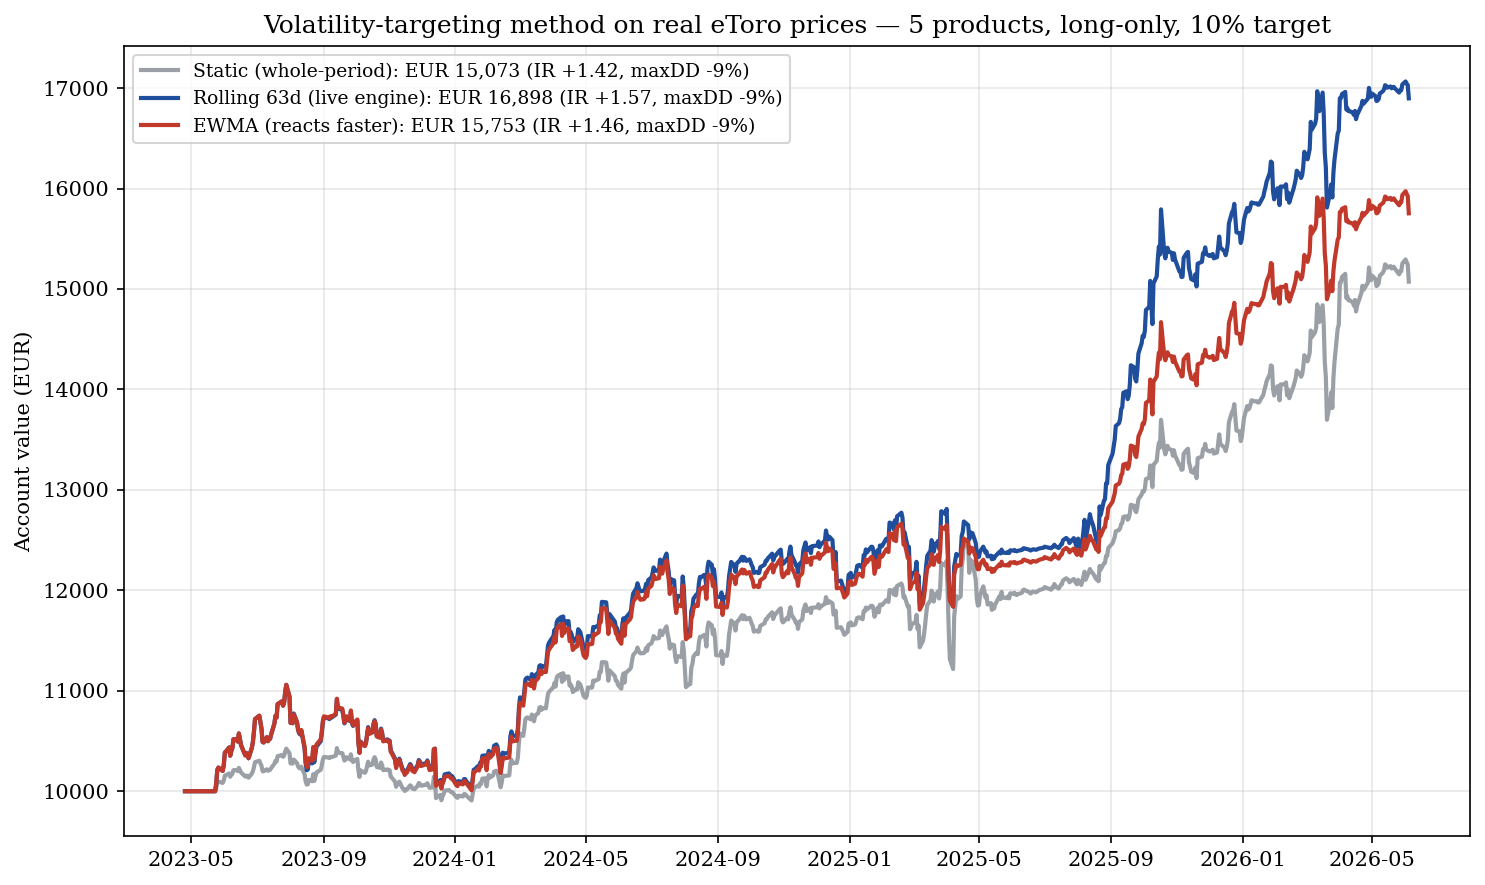
\includegraphics[width=.86\linewidth]{fig_etoro_vol_methods.png}
\caption{Στατικός, κυλιόμενος και EWMA, ο ένας πάνω στον άλλο. Ίδια βουτιά και για τους τρεις· ο
κυλιόμενος (μπλε), δηλαδή αυτός που τρέχει ζωντανά, βγήκε λίγο μπροστά.}\end{figure}

\section{Νικώντας το «αγοράζω και κρατάω»}

Μια δίκαιη ένσταση είναι ότι, σε μια ανοδική δεκαετία, το σκέτο «αγοράζω και κρατάω» έβγαλε πολλά. Είναι
αλήθεια --- αλλά με τεράστιο ρίσκο, με βουτιά που έφτασε το 34\%. Το ωραίο είναι ότι δεν χρειάζεται να
διαλέξουμε. Με μια τεχνική που λέγεται return stacking κρατάμε τις μετοχές \emph{και} προσθέτουμε τη
στρατηγική από πάνω με λίγη μόχλευση, και έτσι ξεπερνάμε το σκέτο «αγοράζω και κρατάω», με καλύτερη
μάλιστα ποιότητα.

\begin{figure}[ht]\centering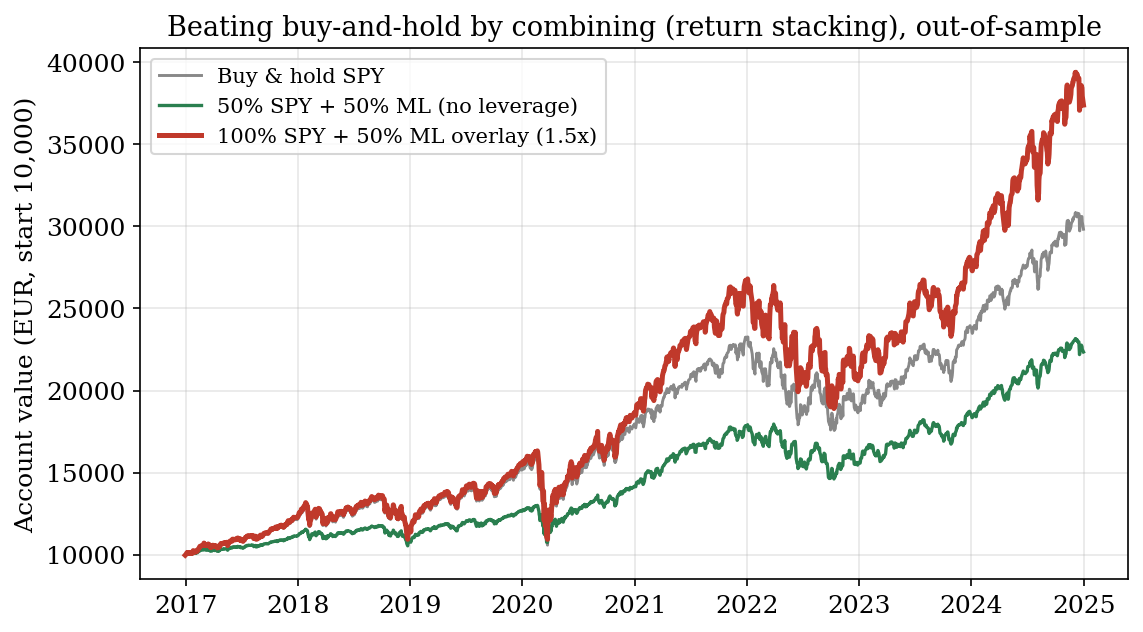
\includegraphics[width=.82\linewidth]{fig_beat_buyhold.png}
\caption{Κρατώντας τις μετοχές και προσθέτοντας τη στρατηγική από πάνω, ο λογαριασμός φτάνει τα
37.390\eur{} έναντι 29.825\eur{} του σκέτου «αγοράζω και κρατάω» --- και με καλύτερο Sharpe.}\end{figure}

\section{Το νευρωνικό μοντέλο}

Στη μεγάλη δοκιμή των δεκαεπτά ετών, το νευρωνικό μοντέλο ξεπέρασε τον σταθερό κανόνα σε ποιότητα
κέρδους. Δεν μιλάμε για κάποιο θαύμα --- το πλεονέκτημα είναι υπαρκτό αλλά μετρημένο, και προτιμώ να το
παρουσιάσω έτσι παρά να το φουσκώσω. Στατιστικά, το σήμα του ML δεν είναι τύχη (ο δείκτης Newey-West
βγαίνει περίπου 2 και ο Deflated Sharpe γύρω στο 0.67), αλλά ούτε και εκκωφαντικό.

\begin{table}[ht]\centering\small
\begin{tabular}{lrrrr}\toprule
Στρατηγική & Sharpe & Ετήσιο & Χειρ. πτώση & 10.000\eur{} $\to$ \\\midrule
Σταθερός κανόνας & 0.47 & $+4.3\%$ & $-21\%$ & 13.978\eur{} \\
\textbf{Νευρωνικό (LSTM)} & \textcolor{good}{0.58} & $+5.4\%$ & $-17\%$ & 15.274\eur{} \\
Αγοράζω και κρατάω SPY & 0.84 & $+14.7\%$ & $-34\%$ & 29.825\eur{} \\
\textbf{Μετοχές + στρατηγική από πάνω} & \textcolor{good}{\textbf{0.98}} & $+18.0\%$ & $-33\%$ & \textcolor{good}{\textbf{37.390\eur{}}} \\
\bottomrule\end{tabular}
\caption{Δεκαεπτά χρόνια, εκτός δείγματος, μετά κόστη.}
\end{table}

\begin{figure}[ht]\centering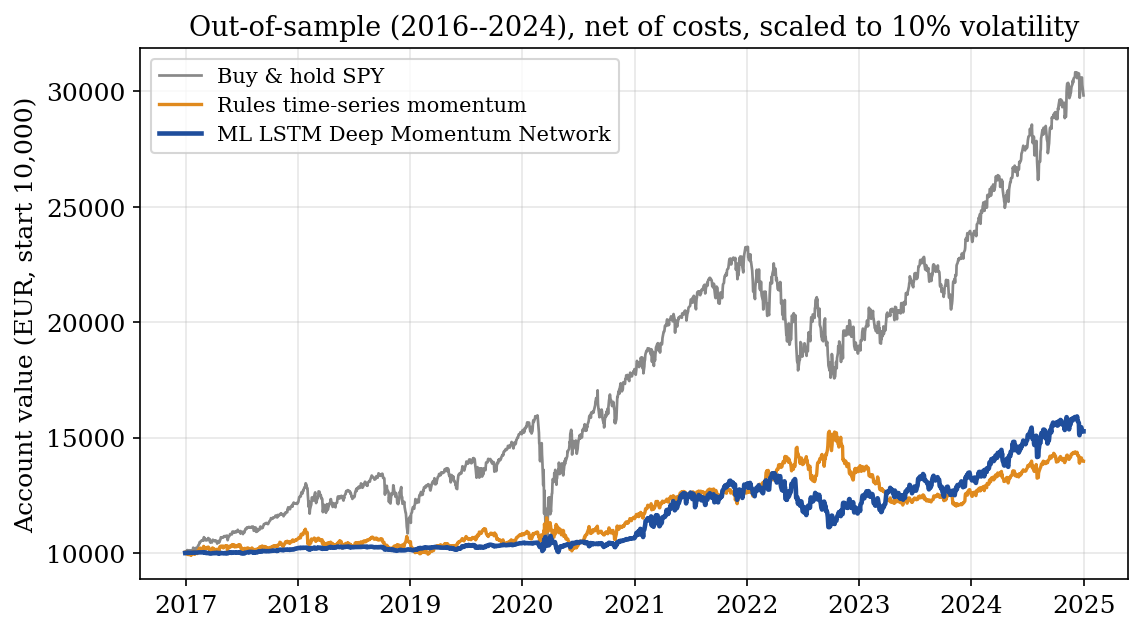
\includegraphics[width=.82\linewidth]{fig_ml_equity.png}
\caption{Το νευρωνικό (μπλε) ξεπερνά τον σταθερό κανόνα (πορτοκαλί). Το «αγοράζω και κρατάω SPY» (γκρι)
έβγαλε περισσότερα σε αυτή την ανοδική περίοδο, αλλά με πολύ μεγαλύτερο ρίσκο.}\end{figure}

\section{Πώς συμπεριφέρεται σε πλάγια (sideways) αγορά}

Μια δίκαιη ερώτηση είναι τι κάνει το σύστημα όταν η αγορά δεν έχει τάση, αλλά κινείται πλάγια μέσα σε
ένα εύρος. Αυτό είναι, ιστορικά, το αδύναμο σημείο κάθε στρατηγικής που ακολουθεί τάσεις: χωρίς σαφή
κατεύθυνση, ένας απλοϊκός κανόνας αγοράζει και πουλάει συνεχώς σε ψεύτικα σήματα και χάνει σε προμήθειες.
Ελέγξαμε αν το δικό μας σύστημα το αποφεύγει. Χωρίσαμε τις πραγματικές ημέρες eToro σε τρία καθεστώτα ---
πλάγια, ανάμεικτη, με τάση --- με ένα αντικειμενικό κριτήριο που μετράει πόσο «καθαρή» ήταν η κίνηση, και
συγκρίναμε έναν απλοϊκό κανόνα τάσης με τη δική μας θέση, που μικραίνει όταν η τάση είναι αβέβαιη.

\begin{table}[ht]\centering\small
\resizebox{\linewidth}{!}{%
\begin{tabular}{lrrrr}\toprule
Καθεστώς & Έκθεση απλοϊκού & Έκθεση \textbf{μοντέλου} & Αποτέλεσμα απλοϊκού & Αποτέλεσμα \textbf{μοντέλου} \\\midrule
\textbf{Πλάγια} & $0{,}17$ & \textcolor{good}{\textbf{$0{,}08$}} & \textcolor{warn}{$-0{,}7\%$} & \textcolor{good}{\textbf{$+1{,}1\%$}} \\
Ανάμεικτη & $0{,}19$ & $0{,}10$ & $+1{,}6\%$ & $+0{,}4\%$ \\
Με τάση & $0{,}24$ & $0{,}13$ & $-1{,}9\%$ & $-1{,}5\%$ \\
\bottomrule\end{tabular}}
\caption{Συμπεριφορά ανά καθεστώς (πραγματικές τιμές eToro, πέντε προϊόντα). Στην πλάγια αγορά το
μοντέλο κρατά \emph{τη μισή} έκθεση του απλοϊκού κανόνα και μετατρέπει τη μικρή ζημιά του σε ελαφρώς
θετικό --- αμύνεται αντί να επιτίθεται.}
\end{table}

\begin{figure}[ht]\centering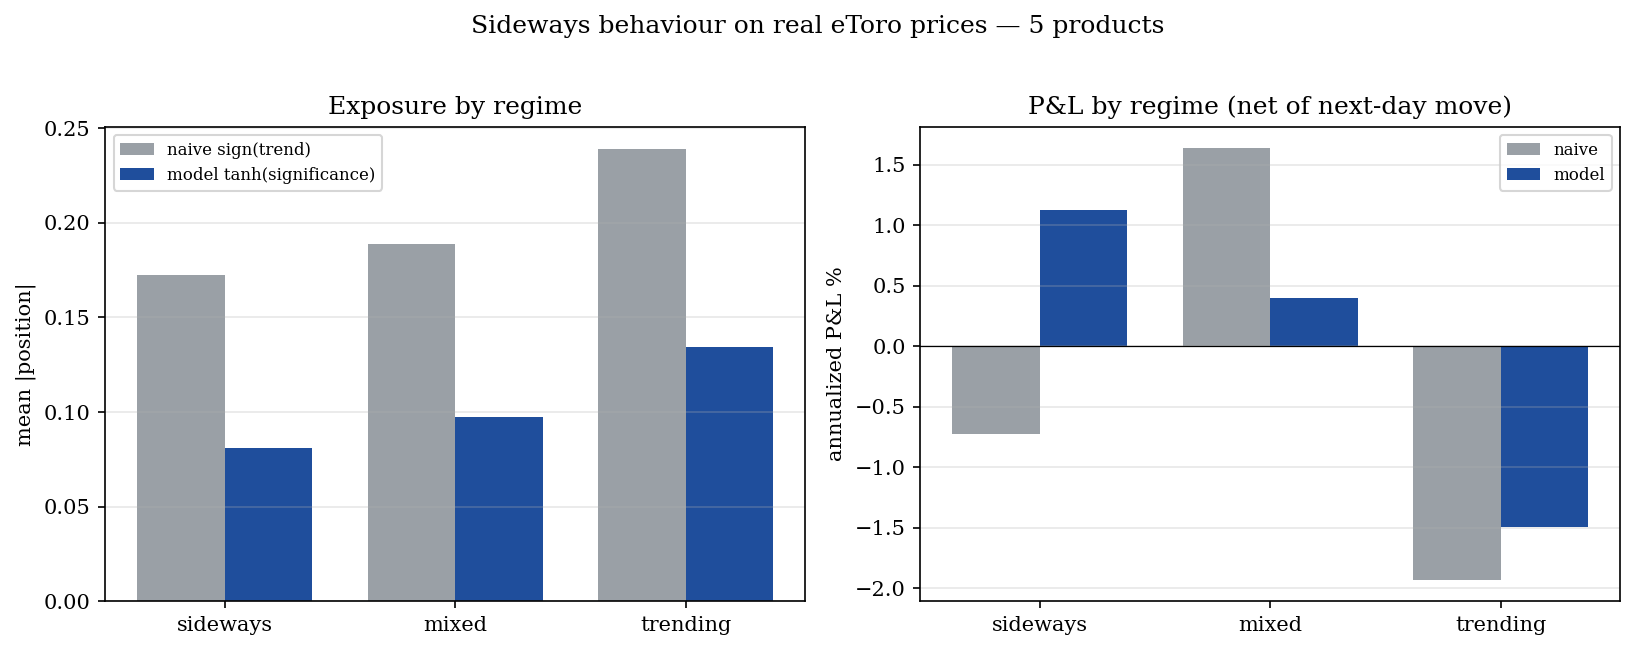
\includegraphics[width=.95\linewidth]{fig_sideways.png}
\caption{Αριστερά: η έκθεση ανά καθεστώς --- το μοντέλο (μπλε) κρατά μικρότερη θέση από τον απλοϊκό
κανόνα (γκρι) παντού, με τη μεγαλύτερη διαφορά στην πλάγια αγορά. Δεξιά: το αποτέλεσμα ανά καθεστώς.}
\end{figure}

Το συμπέρασμα είναι καθαρό αλλά πρέπει να ειπωθεί τίμια. Στην πλάγια αγορά το σύστημα \textbf{μαζεύει
έκθεση} (μισή θέση, λιγότερες συναλλαγές) και έτσι \textbf{αποφεύγει τη ζημιά} που παθαίνει ο απλοϊκός
κανόνας. Δεν \emph{κερδίζει} όμως από το εύρος --- δεν είναι στρατηγική που αγοράζει στον πάτο και πουλάει
στην κορυφή ενός καναλιού. Με δυο λόγια, σε πλάγια αγορά \textbf{αμύνεται}, δεν επιτίθεται.

\aside{Στην τελευταία γραμμή («με τάση») το αποτέλεσμα της επόμενης ημέρας βγαίνει ελαφρώς αρνητικό και
για τις δύο εκδοχές. Αυτό συμβαίνει επειδή το κριτήριο κοιτάζει το \emph{παρελθόν}: μια πολύ «καθαρή»
ανοδική ή καθοδική κίνηση συχνά κάνει μια μικρή \emph{διόρθωση} την αμέσως επόμενη μέρα. Τα νούμερα εδώ
είναι απλοποιημένα (ανά προϊόν, χωρίς το πλήρες χαρτοφυλάκιο) και δείχνουν \emph{συμπεριφορά}, όχι
απόδοση --- τα κανονικά αποτελέσματα είναι αυτά των προηγούμενων ενοτήτων.}

\section{Πόσα ποντάρουμε κάθε φορά}

Πέρα από το τι αγοράζουμε, μετράει και το πόσο. Δοκιμάσαμε αρκετούς τρόπους κατανομής του κεφαλαίου, από
τον απλό «αντιστρόφως ανάλογο της μεταβλητότητας» μέχρι πιο σύνθετους. Όλοι βελτιώνουν λίγο την ποιότητα,
αλλά αυτός που ανεβάζει αισθητά το κέρδος είναι η ελεγχόμενη μόχλευση τύπου Kelly --- με το κόστος,
φυσικά, μεγαλύτερης βουτιάς. Πάλι το ίδιο μάθημα: ρίσκο και κέρδος πάνε μαζί.

\begin{table}[ht]\centering\small
\begin{tabular}{lrrrr}\toprule
Τρόπος κατανομής & Sharpe & Ετήσιο & Χειρ. πτώση & 10.000\eur{} $\to$ \\\midrule
Inverse-vol (βασικό) & 0.44 & $+3.9\%$ & $-19\%$ & 13.603\eur{} \\
HRP (ιεραρχικό) & 0.47 & $+4.3\%$ & $-28\%$ & 14.009\eur{} \\
Min-variance & 0.52 & $+4.8\%$ & $-23\%$ & 14.571\eur{} \\
\textbf{Μόχλευση Kelly (¼)} & \textcolor{good}{0.58} & $+9.2\%$ & $-30\%$ & \textcolor{good}{\textbf{20.268\eur{}}} \\
\bottomrule\end{tabular}
\caption{Τρόποι «πονταρίσματος» στη 17ετή δοκιμή.}
\end{table}

\section{Γιατί δουλεύει εδώ, ενώ στις μετοχές όχι}

Εδώ είναι η καρδιά της εργασίας, και η πιο τίμια διαπίστωσή της. Η ίδια ιδέα της τάσης, αν την
εφαρμόσεις «εγκάρσια» μέσα στις μετοχές --- αγοράζοντας τις δυνατές και πουλώντας τις αδύναμες ---
είναι ουσιαστικά \textbf{νεκρή} σήμερα: μετά τα κόστη δεν βγάζει τίποτα, και μάλιστα προσθέτοντας τον
ανιχνευτή αλλαγής χειροτερεύει. Ζωντανεύει μόνο όταν την εφαρμόσεις \textbf{ανά προϊόν, σε ένα
διαφοροποιημένο καλάθι}. Γι' αυτό όλη μας η προσοχή πήγε στο να διαλέγουμε διαφορετικές κατηγορίες
περιουσιακών στοιχείων, αντί για περισσότερες μετοχές.

\begin{table}[ht]\centering\small
\begin{tabular}{lrrl}\toprule
Προσέγγιση (17ετής, μετά κόστη) & IR & Newey-West t & Ετυμηγορία \\\midrule
Cross-sectional στις μετοχές & \textcolor{warn}{$-0.16$} & $-0.77$ & \textcolor{warn}{νεκρό} \\
\quad + ανιχνευτής αλλαγής μόνος του & \textcolor{warn}{$-1.26$} & $-6.42$ & \textcolor{warn}{χειρότερο} \\
\textbf{Time-series σε διαφοροποιημένο καλάθι} & \textcolor{good}{θετικό} & \textcolor{good}{σημαντικό} & \textcolor{good}{ζωντανό} \\
\bottomrule\end{tabular}
\caption{Η ίδια ιδέα: νεκρή στις μετοχές, ζωντανή στο διαφοροποιημένο καλάθι.}
\end{table}

\begin{figure}[ht]\centering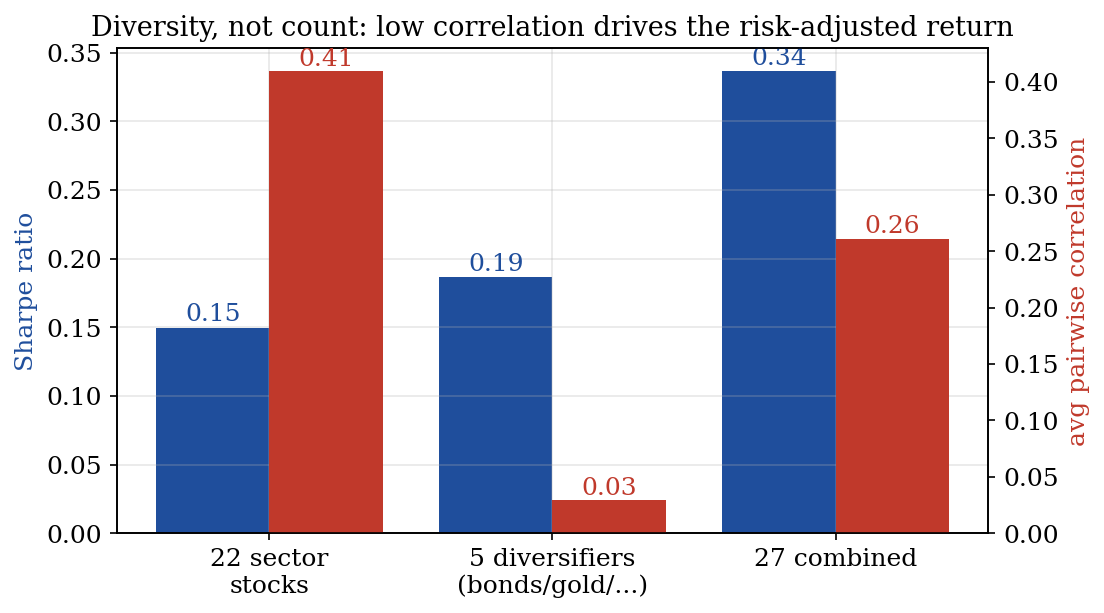
\includegraphics[width=.80\linewidth]{fig_diversification.png}
\caption{Πέντε πραγματικά διαφορετικά πράγματα νικούν εκατό όμοιες μετοχές. Ο συνδυασμός έχει καλύτερο
Sharpe από κάθε κομμάτι του χωριστά --- αυτό είναι το δομικό πλεονέκτημα της διαφοροποίησης.}\end{figure}

\section{Η μεγάλη εικόνα και τι να προσέχουμε}

Για να κλείσω, αξίζει να δει κανείς πώς συμπεριφέρθηκε το σύστημα σε μια πραγματική κρίση. Στο κραχ του
2022 σόρταρε σχεδόν τα πάντα και κράτησε θέσεις αγοράς μόνο στο δολάριο και την ενέργεια --- ακριβώς τα
δύο πράγματα που άντεξαν εκείνη τη χρονιά --- και έτσι προστάτεψε το κεφάλαιο.

\begin{figure}[ht]\centering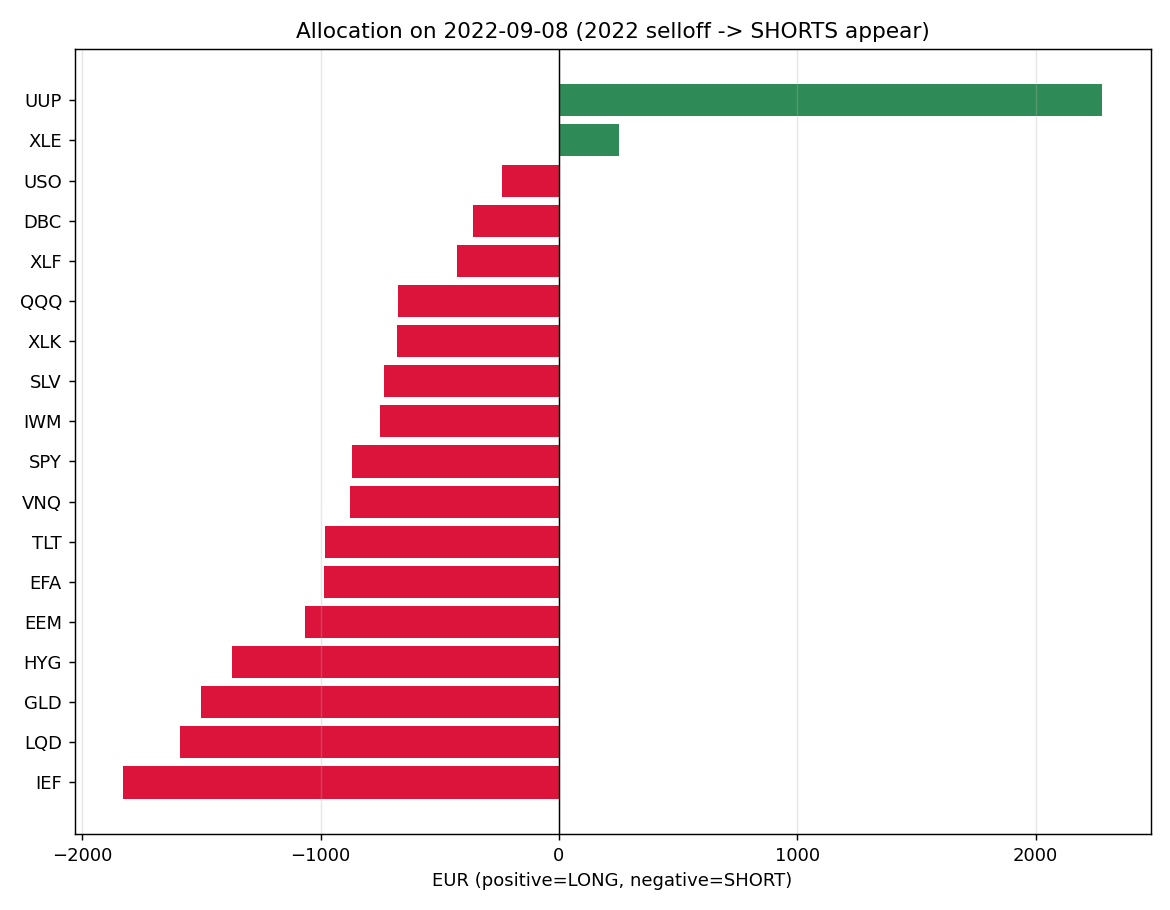
\includegraphics[width=.80\linewidth]{bt_alloc_2022crisis.png}
\caption{Η κατανομή στο κραχ του 2022. Το πράσινο είναι θέσεις αγοράς, το κόκκινο πωλήσεις: το σύστημα
γύρισε αμυντικό μόνο του.}\end{figure}

Οφείλω όμως να κλείσω με μερικές ειλικρινείς προειδοποιήσεις, γιατί χωρίς αυτές το κείμενο θα ήταν
παραπλανητικό. Ένα backtest δεν είναι το μέλλον· είναι δοκιμή στο παρελθόν και δεν εγγυάται τίποτα. Τα
σήματα αυτά εξαρτώνται από το καλάθι και την περίοδο, και σε άλλη εποχή μπορεί να αποδώσουν αλλιώς --- γι'
αυτό άλλωστε ο τίτλος της εργασίας επιμένει στη λέξη «honest». Όλα τα νούμερα είναι μετά από ένα ρεαλιστικό
κόστος συναλλαγών, αλλά οι πραγματικές χρεώσεις μπορεί να διαφέρουν. Το stop-loss, που πολλοί θεωρούν
αυτονόητο, το δοκιμάσαμε και αποδείχθηκε ζημιογόνο: ένα σφιχτό όριο της τάξης του 8\% μείωσε την ποιότητα
και αύξησε τη χειρότερη βουτιά, επειδή πουλάει πάνω στον θόρυβο και χάνει την ανάκαμψη. Το ρίσκο το
ελέγχουμε αλλιώς --- με τη διαφοροποίηση, με το κουμπί ρίσκου και με τον ανιχνευτή αλλαγής. Και, το
πιο σημαντικό, βρισκόμαστε ακόμη σε φάση demo: πραγματικά χρήματα είναι εκτός σκοπού προς το παρόν.

\vfill
\noindent\rule{\linewidth}{0.4pt}\\[2pt]
{\small QUANTIQ \,/\, AGEL AI. Μεθοδολογία: \paperref. Όλα τα μεγέθη είναι καθαρά μετά κόστη και
εκτός δείγματος. Τα ιστορικά αποτελέσματα δεν εγγυώνται μελλοντικές αποδόσεις. Φάση demo.}

\end{document}
